\section{Nonlinear plume-scale climate effects}
As detailed in the previous section, the global contributions to aviation radiative forcing have been relatively well quantified. However, much of the modelling processes used to estimate these contributions are derived from global models assuming instant dispersion, thus excluding subgrid-scale chemical and physical effects that occur in the first 2--12~h upon release into the atmosphere. This section reviews current scientific understanding of these plume-scale processes, and highlights their emerging relevance in increasingly high-density airspace regions, as the accumulation of chemically active emission species further propagates the nonlinear atmospheric response.

\subsection{Gas-phase photochemistry}
\label{Gas-phase_photochem}
The ultimate chemical composition of the troposphere is largely influenced by the removal of natural and anthropogenic trace species (e.g. \ce{CH_4}, CO, \ce{O_3}) through oxidation reactions with atmospheric free radicals, primarily the hydroxyl radical (\ce{OH}), which are relatively short-lived and in low concentrations owing to their fast reactivity \cite{Stone2012, Monks2005}. The relative abundance of OH in the troposphere controls the degree of removal of ambient trace species, otherwise known as the atmosphere's oxidative capacity. In the purely hypothetical situation where gas-phase radical chemistry was absent and hence the oxidative capacity of the atmosphere was zero, the levels of many harmful pollutants would continue to rise unabated, resulting in a drastic change in the chemical, biological and radiative state of the Earth-atmosphere system \cite{Prinn2003}. OH is produced via atmospheric photochemistry and photolysis; sunlight-initiated reaction of photolabile molecules to produce highly reactive species and/or radical species. Ozone is photolysed by ultraviolet light ($\lambda <$ 320~nm) to produce excited singlet oxygen \ce{O(^{1}D)} \eqref{O3+hv}, which then produces two hydroxyl radicals in the presence of sufficient levels of water vapour \eqref{O1D+H2O}. The symbol M represents a non-reacting molecule in the equation, that has the role of absorbing reaction energy to create stable products.

\reaction[O3+hv]{O_3 + h\nu  (\lambda \ $<$  320 nm) -> O(^1D) + O_2}

\reaction[O1D+H2O]{O(^1D) + H_2O -> OH + OH}

Understanding the influence of OH and the oxidative capacity of the upper troposphere is critical for the environmental analysis of aircraft emissions, as the closely-coupled chemical scheme involving hydroxyl and hydroperoxy radicals ($\ce{HO_x} = \ce{OH} + \ce{HO_2}$) and nitrogen oxides ($\ce{NO_x} = \ce{NO} + \ce{NO_2}$) determines the production and loss of key climate forcing species such as ozone and methane.

Most oxidation processes that occur in the troposphere are photochemical reaction schemes involving \ce{HO_x}, and are therefore only applicable in daylight conditions due to the reliance on solar actinic flux \cite{Jacobson2005}. There is however, a range of chemical processes mainly involving nitrate radicals, that are potentially important for nighttime tropospheric oxidation processes involving key climate forcing species. See Jenkin et al.\ (2000) \cite{Jenkin2000} for further elaboration on nighttime tropospheric chemistry.

\begin{figure}[H]
	\centering
	\subfloat
		{
		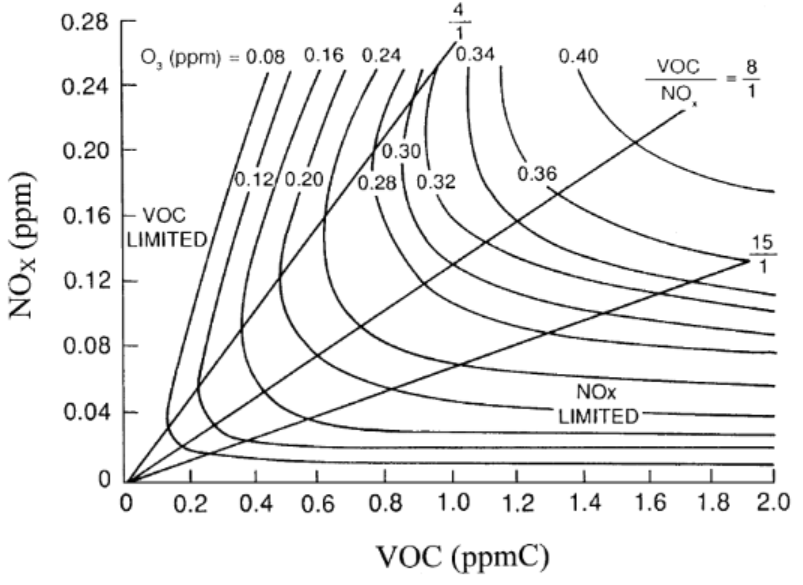
\includegraphics[width=.38\textwidth]{NOx-VOC_curve.png}
		\vspace{.2cm}
		\label{NO_x_VOC}
		}
	\subfloat
		{
		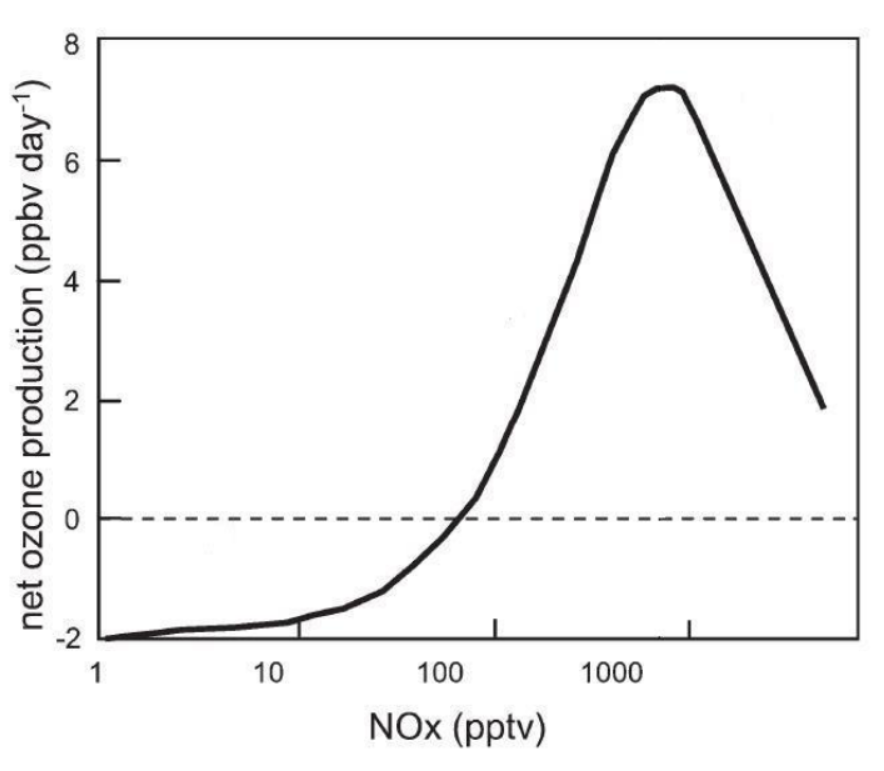
\includegraphics[width=.32\textwidth]{NO_x_ozone.png}
		\label{NO_x_ozone}
		}
	\caption{\textbf{(a)} Example isopleth diagram displaying peak ozone concentrations calculated from various initial concentrations of \ce{NO_x} and a specified VOC mixture, using the US EPA empirical kinetic model \cite{Dodge1977, Jenkin2000}. \textbf{(b)} Schematic representation of the variation of net ozone production efficiency with \ce{NO_x} concentrations, with magnitudes reflecting clean free tropospheric conditions (i.e. low VOC/\ce{NO_x} ratio) \cite{Monks2005}.}
	\label{}
\end{figure}

Figure \ref{NO_x_VOC} from Jenkin et al.\ (2000) \cite{Jenkin2000} is an exemplary ozone isopleth diagram that illustrates the \ce{O_3}-\ce{NO_x}-VOC relationship. At typical aircraft cruising altitudes (i.e. UTLS), where the emissions of \ce{NO_x} have a significant influence on atmospheric chemistry, it is likely that VOC content is very low relative to the background NO and \ce{NO_2} concentrations. Therefore, it is likely that typical VOC/\ce{NO_x} ratios are low in the UTLS, meaning that under the assumption of constant VOC concentrations, the \ce{NO_x}-\ce{O_3} relationship takes a form similar to figure \ref{NO_x_ozone}.

\subsubsection{Low-\ce{NO_x} regime}
In unpolluted environments characterised by low \ce{NO_x} concentrations, such as in regions where the ambient air is unperturbed by aircraft emissions, the dominant reaction pathway of OH is to react with CO (\textasciitilde75\%), with the remainder reacting with \ce{CH_4} \cite{Thompson1992}. The dominant reaction pathway therefore involves the oxidation of CO to form \ce{CO_2}, as in reaction \eqref{OH+CO} (for a detailed description of both the CO and the \ce{CH_4} oxidation cycles in low \ce{NO_x} conditions, see Wasiuk (2014) \cite{Wasiuk2014}). In this CO oxidation cycle, produced atomic hydrogen (H) then reacts with oxygen to form \ce{HO_2} \eqref{H+O2+M}, which subsequently reacts with \ce{O_3} to form OH in the background troposphere \eqref{HO2+O3}. This initiates a chain sequence in which OH and \ce{HO_2} interconvert through the termination of ozone \eqref{OH+O3}. This clean condition scheme therefore limits pollutant build up in the unpolluted upper troposphere and keeps ozone levels under control \cite{Jacob1999}.

\reaction[OH+CO]{OH + CO -> H + CO_2}

\reaction[H+O2+M]{H + O_2 + M -> HO_2 + M}

\reaction[HO2+O3]{HO_2 + O_3 -> OH + 2O_2}

\reaction[OH+O3]{OH + O_3 -> HO_2 + O_2}

Net reaction: \reaction[CO+O3->CO2+O2]{OH + CO + 2O_3 -> CO_2 + HO_2 + 2O_2}

Alternatively, \ce{HO_2} can react with itself to form hydrogen peroxide (\ce{H_2O_2}) \eqref{HO2+HO2}, or with organic peroxy radicals such as the methyl peroxy radical (\ce{CH_3O_2}) to form organic hydroperoxides \eqref{CH3O2+HO2}. These reaction pathways can become an effective sink for \ce{HO_x} under most conditions, because the formation of peroxides prevents further \ce{HO_x} interconversion \cite{Gunz1990}.

\reaction[HO2+HO2]{HO_2 + HO_2 + M -> M + O_2 + H_2O_2}

\reaction[CH3O2+HO2]{CH_3O_2 + HO_2 -> CH_3O_2H + O_2}

\subsubsection{\ce{NO_x}-limited regime}
In polluted environments, where \ce{NO_x} levels are raised considerably above ambient concentrations (e.g. typical aircraft cruising altitudes), CO oxidation takes place through reactions \eqref{OH+CO} \eqref{H+O2+M}, however in the presence of nitrogen oxides, ozone is produced rather than depleted. Peroxide formation reactions \eqref{HO2+HO2} and \eqref{CH3O2+HO2} compete with the oxidation of NO to \ce{NO_2} \eqref{HO2+NO} for available \ce{HO_2} concentrations. When the latter reaction prevails, \ce{NO_2} photolysis takes place, converting back to NO with ground state oxygen \ce{O(^{3}P)} forming as a byproduct \eqref{NO2+hv}. Subsequently, \ce{O(^{3}P)} reacts with atmospheric oxygen to produce \ce{O_3} \eqref{O3P+O2+M}.

\reaction[HO2+NO]{HO_2 + NO -> OH + NO_2}

\reaction[NO2+hv]{NO_2 + h\nu (\lambda $<$ 420 nm) -> NO + O(^3P)}

\reaction[O3P+O2+M]{O(^3P) + O_2 + M -> O_3 + M}

Net reaction: \reaction[CO+2O2]{CO + 2O_2 -> CO_2 + O_3}

Additionally, the methane oxidation cycle leads to net ozone production in the presence of \ce{NO_x}. The oxidation of methane by OH produces water vapour and the methyl radical (\ce{CH_3}) \eqref{OH+CH4}, which further reacts with oxygen to form \ce{CH_3O_2} \eqref{CH3+O2+M}. The produced methyl peroxy radical can then react with \ce{NO} to form \ce{NO_2} through reaction \eqref{CH3O2+NO}.

\reaction[OH+CH4]{OH + CH_4 -> H_2O + CH_3}

\reaction[CH3+O2+M]{CH_3 + O_2 + M -> M + CH_3O_2}

\reaction[CH3O2+NO]{CH_3O_2 + NO -> CH_3O + NO_2}

\reaction[CH3O+O2]{CH_3O + O_2 -> HO_2 + HCHO}

Net reaction: \reaction[CH4+2O2]{CH_4 + 2O_2 -> HCHO + O_3}

The methoxy radical (\ce{CH_3O}) produced can form additional \ce{HO_2} and formaldehyde (HCHO) through reaction \eqref{CH3O+O2}, which is then capable of reacting to form further \ce{NO_2} through reaction \eqref{HO2+NO}. The resultant \ce{NO_2} produced through reactions \eqref{CH3O2+NO} and \eqref{HO2+NO} consequently produces ozone through the same pathway as CO oxidation (i.e. \ce{NO_2} photolysis \eqref{NO2+hv} followed by reaction of the \ce{O(^3P)} photoproduct \eqref{O3P+O2+M}). The net reaction of methane oxidation in polluted environments therefore results in positive ozone production. Figure \ref{NOx-O3-CO-CH4} is a visual representation of the \ce{NO_x}-\ce{O_3}-CO-\ce{CH_4} oxidation reaction scheme described thus far.

\begin{figure}[H]
  \centering
  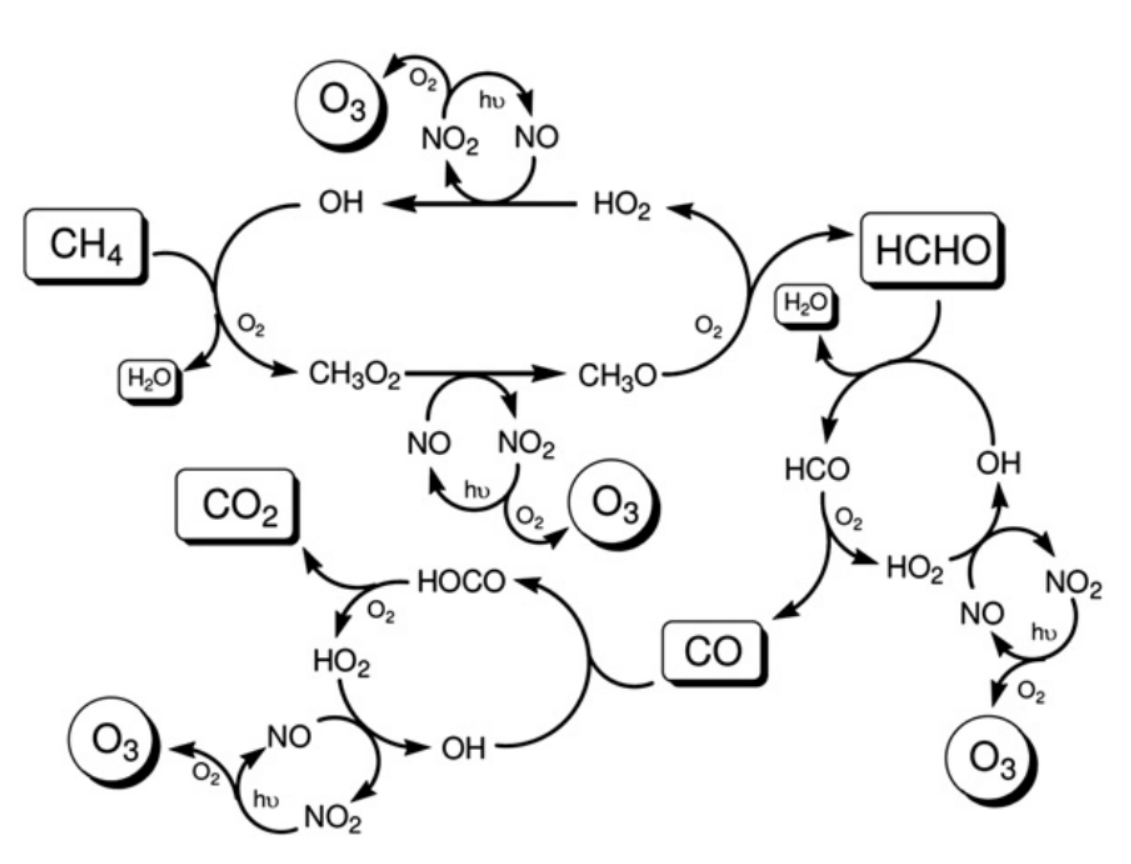
\includegraphics[width=0.65\linewidth]{NOx-O3-CO-CH4.png}
  \caption{Schematic representation of the OH initiated, \ce{NO_x}-catalysed oxidation scheme for CO and \ce{CH_4} \cite{Jenkin2008}.}
  \label{NOx-O3-CO-CH4}
\end{figure}


%The resultant \ce{NO_2} produced from reaction \eqref{} can then feed into the ozone formation cycle through \eqref{} and \eqref{}. Alternatively, the methoxy radical (\ce{CH_3O}) produced can form additional \ce{HO_2} and formaldehyde (HCHO) through reaction \eqref{}, which then produces further \ce{NO_2} through 

%Ozone role in oxidation of atmosphere. How it leads to warming. How aircraft NOx increases ozone production rate.

\subsubsection{\ce{NO_x}-saturated regime}
Under very high \ce{NO_x} conditions, such as inside aircraft exhaust plumes or in regions of the atmosphere where aircraft fly in close proximity and their corresponding emissions accumulate, the ozone production efficiency starts to drop off. This is because as NO and \ce{NO_2} surpass a threshold concentration, known as the compensation point (peak of the curve in figure \ref{NO_x_ozone}), they begin to compete with VOCs (e.g. methane) for reaction with hydroxyl (OH), organic peroxy (\ce{RO_2}) and peroxide \ce{RCO_3} radicals \cite{Wasiuk2014}. The products of these reactions are examples of nitrogen reservoir species: nitrous acid (HONO), nitric acid (\ce{HNO_3}), peroxynitric acid (\ce{HO_2NO_2}), peroxy nitrates (\ce{RO_2NO_2}) and peroxyacyl nitrates (\ce{RCO_3NO_2}). Reservoir species are much less efficient at forming ozone as they are more stable and are also more likely to get washed out of the atmosphere through depositional processes \cite{Jenkin2000}. They are also much more stable in the upper troposphere compared to the surface equivalent \cite{Khan2020}. Thus, reactions \eqref{NO+OH+M} to \eqref{NO2+RCO3+M} serve as termination reactions, removing radicals from the atmosphere and preventing additional ozone formation through conversion of \ce{NO_x} to its more stable counterparts.

\reaction[NO+OH+M]{NO + OH + M -> HONO + M}
\reaction[NO2+OH+M]{NO_2 + OH + M -> HNO_3 + M}
\reaction[NO2+HO2+M]{NO2 + HO_2 + M -> HO_2NO_2 + M}
\reaction[NO2+RO2+M]{NO_2 + RO_2 + M -> RO_2NO_2 + M}
\reaction[NO2+RCO3+M]{NO_2 + RCO_3 + M -> RCO_3NO_2 + M}

\ce{NO_x} saturation effects become particularly important to observe in the case of diluting aircraft exhaust plumes, because the high \ce{NO_X}-VOC ratio means that termination reactions are often favoured over catalytic ozone formation \cite{Song2003}. In the relatively fresh exhaust plume (first 10 minutes) where \ce{NO_x} concentrations are significantly enhanced, ozone titration by NO results in large scale production of \ce{NO_2} \eqref{NO+O3}, but decreases the formation of \ce{HO_x} due to depleted ozone levels in the plume.

\reaction[NO+O3]{NO + O_3 -> NO_2 + O_2}

The dilution of the plume results in reduced \ce{NO_x} concentrations over time, and the in-plume chemistry transitions from \ce{NO_x}-saturated to \ce{NO_x}-limited. With ozone levels still depleted, the remaining \ce{HO_2} and \ce{RO_2} in the plume (formed from the oxidation of CO and VOCs by OH) react with the remaining NO to produce OH and \ce{NO_2} without further depleting ozone. This leads to increasing OH and \ce{NO_2} concentrations which give rise to a net ozone recovery due to \ce{NO_2} photolysis (reactions \eqref{NO2+hv} and \eqref{O3P+O2+M}), with full recovery to ambient concentrations within 1--2~h post emission. As ozone levels rise in the plume back towards ambient concentrations, the photochemical formation of OH becomes more common, through reactions \eqref{O3+hv} and \eqref{O1D+H2O}. Newly formed OH can oxidise CO and VOCs to form peroxy radicals which catalyse ozone production, however it can also react with NO and \ce{NO_2} to form stable nitrogen reservoir species, through reactions \eqref{NO+OH+M} to \eqref{NO2+RCO3+M} \cite{Fritz2020}.

In the ID scenario inherent to large-scale climate models, ozone titration doesn't occur on the same scale due to lower mixing ratios of \ce{NO_x} when instantly diluted. Therefore, initial ozone depletion and subsequent recovery in the exhaust plume is not properly captured, meaning that instead, ozone levels remain reasonably high throughout and hence \ce{HO_x} production can remain stable. The stable \ce{HO_x} levels mean \ce{NO_x} to reservoir species conversion remains stable also, throughout the \ce{NO_x} lifetime. On a global scale, it has been shown that inclusion of plume processes leads to a net reduction in ozone forming potential of aviation \ce{NO_x} emissions. Vohralik et al.\ (2008) \cite{Vohralik2008} summarises the estimates made for the degree of reduction in ozone forming potential when plume effects were included. Initial findings from Kraabol et al.\ (2002) \cite{Kraabol2002} and Meijer et al.\ (1997) \cite{Meijer1997} estimated discrepancies in ozone production of 15--18\%, however these studies only accounted for ozone depletion in the plume, and not the \ce{O_3} generated during plume expansion. Inclusion of both ozone depletion and production in the plume in Meijer (2001) \cite{Meijer2001}, led to updated estimates in ozone formation changes 0\% to -5\% in January and +5\% to -10\% in July, indicating that plume processing can actually increase net ozone production when propagated to global scales. %Estimates from Fritz?

%The instantaneous dilution assumption inherent to large-scale climate models neglects the initial ozone depletion and subsequent recovery in the exhaust plume, hence omitting the in-plume \ce{NO_x} and \ce{HO_x} depletion, and therefore leading to a relatively constant ozone production rate throughout \cite{Fritz2020}. When propagated to global scales In Vohralik et al.\ (2008) \cite{Vohralik2008}, estimates for 

% Need to talk about different estimates for how much plume leads to overestimation of ozone

\subsection{Heterogeneous chemistry}
Reactions occurring in the atmosphere on either the gas--solid interface (e.g. aerosol particles) or the gas--liquid interface (e.g. cloud droplets) are referred to as heterogeneous reactions. The heterogeneous chemistry which can affect ozone concentrations through production and loss of \ce{HO_x} and \ce{NO_x} and the production of halogen radicals is extremely important in particle rich aircraft exhaust plumes and contrails \cite{Jacob2000}. The exhaust plume contains emitted soot particles and ultrafine aqueous aerosol particles which are either formed within the plume or entrained into the plume from ambient air, as elaborated on in the following subsection. In the case of contrail formation, heterogeneous chemistry becomes very efficient, due to the four-fold increase in particle surface area of contrail ice compared to typical exhaust and background aerosol surface area. Meilinger et al.\ (2005) \cite{Meilinger2005} states that the heterogeneous reactions occurring on aerosol particles have a negligible effect on ozone, however contrail ice can influence the ozone response to aircraft emissions by $\pm$0.5\% on a macroscopic scale which varies depending on time of day and year. Due to the relatively minor impact heterogeneous chemical reactions have on aircraft-induced ozone perturbations, and hence on aviation climate impact, their effect will be acknowledged, but the chemical intricacies will not be discussed further. For more information, see the references contained within this paragraph. 

%The effect of plumes on atmospheric photochemistry is shown to increase the soot, sulphate and water-ice surface areas for heterogeneous reactions which are important in defining ozone removal rates in the UTLS. \ce{N_2O_5} formed from the oxidation of \ce{NO_x} undergoes a reactive uptake on the plume species (e.g. water-ice surface), which results in \ce{HNO_3} formation. The reaction of \ce{N_2O_5} with HCl on ice results in \ce{ClNO_2} formation \eqref{N2O5+HCl->ClNO2+HNO3} which can compete with heterogeneous hydrolysis of N2O5 \eqref{N2O5+H2O->2HNO3}.
%
%\reaction[N2O5+H2O->2HNO3]{N_2O_5 + H_2O -> 2HNO_3}
%
%\reaction[N2O5+HCl->ClNO2+HNO3]{N_2O_5 + HCl -> ClNO_2 + HNO_3}
%
%The heterogeneous interactions are very important to the removal of \ce{NO_x} and \ce{HO_x} species during sedimentation events in the UTLS. These reactions can form reservoir species (e.g. \ce{HNO_3}, \ce{H_2O_2}) which can absorb onto sulphate aerosol and ice particles. Heterogeneous denoxification (reactions \eqref{N2O5+H2O->2HNO3} and \eqref{N2O5+HCl->ClNO2+HNO3}) and dehoxification (reactions \eqref{2HO2->H2O2+O2} and \eqref{2OH->H2O2}) lead to reduced concentrations of \ce{NO_x} and \ce{HO_x} which reduce the ozone production through gas-phase reactions \cite{Meilinger2005}.
%
%\reaction[2HO2->H2O2+O2]{2HO_2 -> H_2O_2 + O_2}
%
%\reaction[2OH->H2O2]{2OH -> H_2O_2}
%
%In the stratosphere, a number of heterogeneous reactions \eqref{ClONO2+H2O->HOCl+HNO3} to \eqref{HOBr+HBr->Br2+H2O} are important to various degrees on the surface of ice particles and saturated ternary solutions of water, HNO3 and H2SO4 in terms of ozone depletion on a global scale.
%
%\reaction[ClONO2+H2O->HOCl+HNO3]{ClONO_2 + H_2O -> HOCl + HNO_3}
%
%\reaction[ClONO2+HCl->Cl2+HNO3]{ClONO_2 + HCl -> Cl_2 + HNO_3}
%
%\reaction[ClONO2+HBr->BrCl+HNO3]{ClONO_2 + HBr -> BrCl + HNO_3}
%
%\reaction[HOCl+HCl->Cl2+H2O]{HOCl + HCl -> Cl_2 + H_2O}
%
%\reaction[HOCl+HBr->BrCl+H2O]{HOCl + HBr -> BrCl + H_2O}
%
%\reaction[BrONO2+H2O->HOBr+HNO3]{BrONO_2 + H_2O -> HOBr + HNO_3}
%
%\reaction[BrONO2+HCl->BrCl+HNO3]{BrONO_2 + HCl -> BrCl + HNO_3}
%
%\reaction[HOBr+HCl->BrCl+H2O]{HOBr + HCl -> BrCl + H_2O}
%
%\reaction[HOBr+HBr->Br2+H2O]{HOBr + HBr -> Br_2 + H_2O}
%
%The heterogeneous reactions initiated by \ce{ClONO_2}, HOCl, \ce{BrONO_2}, HOBr produce \ce{Cl_2}, BrCl, \ce{Br_2} which then yields Cl and Br radicals by photolysis. The heterogeneously activated Cl and Br can subsequently enhance ozone depletion \cite{Meilinger2005}.
%
%The extent of heterogeneous reactions \eqref{N2O5+H2O->2HNO3} to \eqref{HOBr+HBr->Br2+H2O} offset the effects of gas-phase reactions \eqref{NO+O3->NO2+O2} to \eqref{NO2+RCO3+M->RCO3NO2+M} on \ce{NO_x} initiated ozone formation which depends on a variety of chemical and dynamic factors (e.g. aerosol microphysics, atmospheric dynamics).

 \subsection{Aerosol and contrail microphysics}
\label{Microphysics}
Whilst the climate impact of aviation \ce{NO_x} emissions is dependent on the photochemical processes catalysing ozone production and methane destruction, the evolution and radiative forcing of aerosols and contrails is predominantly controlled by microphysical processes that occur at the aircraft plume scale. 

\subsubsection{The microphysical formation of aerosols and contrails}
Upon release into the atmosphere, aerosol particle formation occurs through one of two nucleation pathways: 

\begin{enumerate}
	\item The condensation of two distinct gas phase molecules to form a liquid phase droplet through what is known as binary homogeneous nucleation. This is the case for reactive sulphur emissions that get chemically oxidised into sulphuric acid (\ce{H_2SO_4}), which then condenses with water vapour to form \ce{H_2SO_4 / H_2O} droplets \cite{Perry1994}.
	\item The gas-to-particle conversion occurring on the surface of foreign particles is known as binary heterogeneous nucleation, often leading to a liquid coating that forms on the particle. For example, \ce{H_2SO_4 / H_2O} droplets can form a partial liquid coating around chemically activated soot in the aircraft exhaust plume through heterogeneous nucleation, leading to soot aerosol formation; a process that plays an important role in the formation of contrails \cite{Karcher1996a}.
\end{enumerate}

\begin{figure}[H]
  \centering
  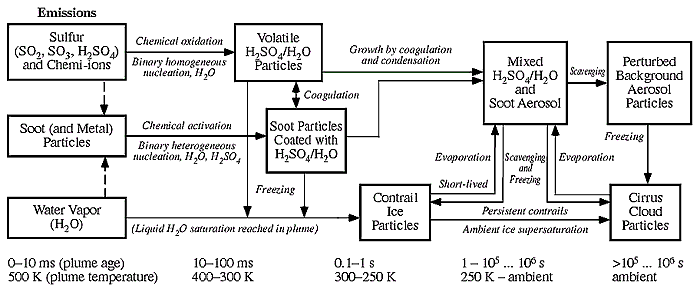
\includegraphics[width=0.95\linewidth]{Aerosol_fig.png}
  \caption{The microphysical formation of aerosol and contrail particles in an aircraft plume. Displayed as a function of plume age and temperature \cite{IPCC1999}.}
  \label{Microphys_IPCC}
\end{figure}

Newly formed aerosol particles subsequently grow in the aircraft wake due to further condensation by uptake of surrounding water vapour, and a process known as coagulation. Coagulation refers to the collision between particles that results in the formation of larger particles, often initiated by graviational settling, turbulence or thermal motion. A process called scavenging occurs when two particles, one much larger than the other, coagulate and lead to the removal of the small particle from its particular size category, with its mass contributing slightly to the increase in mass of the larger particle. Coagulation commonly occurs in aircraft wakes between volatile particles such as \ce{H_2SO_4 / H_2O} particles and soot aerosol, forming a mixed \ce{H_2SO_4 / H_2O}-soot aerosol (see figure \ref{Microphys_IPCC}). This sulphate-soot aerosol may eventually become scavenged by background aerosol particles if it remains stable for up to a day \cite{IPCC1999}. Alternatively, if at any point during the mixing process of aircraft exhaust with air, water-supersaturation is exceeded, aircraft-induced particles and entrained background aerosol can be activated into water droplets through the uptake of surrounding water vapour \cite{Karcher2018}. If temperatures are below threshold according to the SA criterion, then these aerosol-activated water droplets will freeze to form contrail ice particles in the aircraft wake on the order of seconds post emission. 

\subsubsection{Contrail microphysical properties}
The aforementioned microphysical processes (i.e. nucleation, condensation, coagulation, scavenging and freezing) determine the eventual composition and size distribution of particles in the aircraft wake, and if thermodynamic conditions permit, the formation and evolution of contrail ice particles \cite{AIR5715, Karcher2015}. Hereinafter, this section will focus on the microphysics of contrail ice particles, as they induce the most significant radiative response out of all aviation climate forcers. Findings from K{\"a}rcher et al.\ (1996b) \cite{Karcher1996b} conclude that the predominant ice nucleation pathway for contrail formation is heterogeneous freezing of chemically activated soot aerosol particles, as these are the only remaining particle type in sufficient abundance at the time of freezing. However, simulation results from K{\"a}rcher et al.\ (1998) \cite{Karcher1998} strongly suggest that contrail formation is still likely in the absence of soot and sulphur emissions, through the activation and freezing of background aerosols. 

The radiative forcing of contrails is thought to be determined by the product of optical depth and areal coverage \cite{Schumann2017}. In terms of areal coverage, contrail forcing is thus dominated by the presence of persistent contrails and contrail cirrus. However, the optical depth of a contrail is less dependent on its macroscopic properties and is instead determined by the optical and physical characteristics of the ice particles on the microscopic scale. The microphysical parameters deemed to be most responsible for inducing a radiative response are ice water content (amount of cloud ice per unit volume \cite{Karcher2018}), total ice particle number concentration, ice particle size distributions, effective radii, and ice particle shape \cite{Heymsfield2010}. Various studies have formulated methods to estimate RF and ERF from contrails, based on the parametrisation of these properties \cite{Meerkotter1999, Schumann2012a, Bickel2020}. It is defined that the optical depth is proportional to the ice water content divided by the effective radius of entrained ice particles \cite{Schumann2012a}. Contrails that tend to have more aspherical ice particle shapes are likely to have a stronger solar albedo, increasing the reflectance of the SW flux \cite{Meerkotter1999}. Ice number concentration is also thought to increase optical depth \cite{Karcher1999}. 

\begin{figure}[H]
	\centering
	\subfloat
		{
		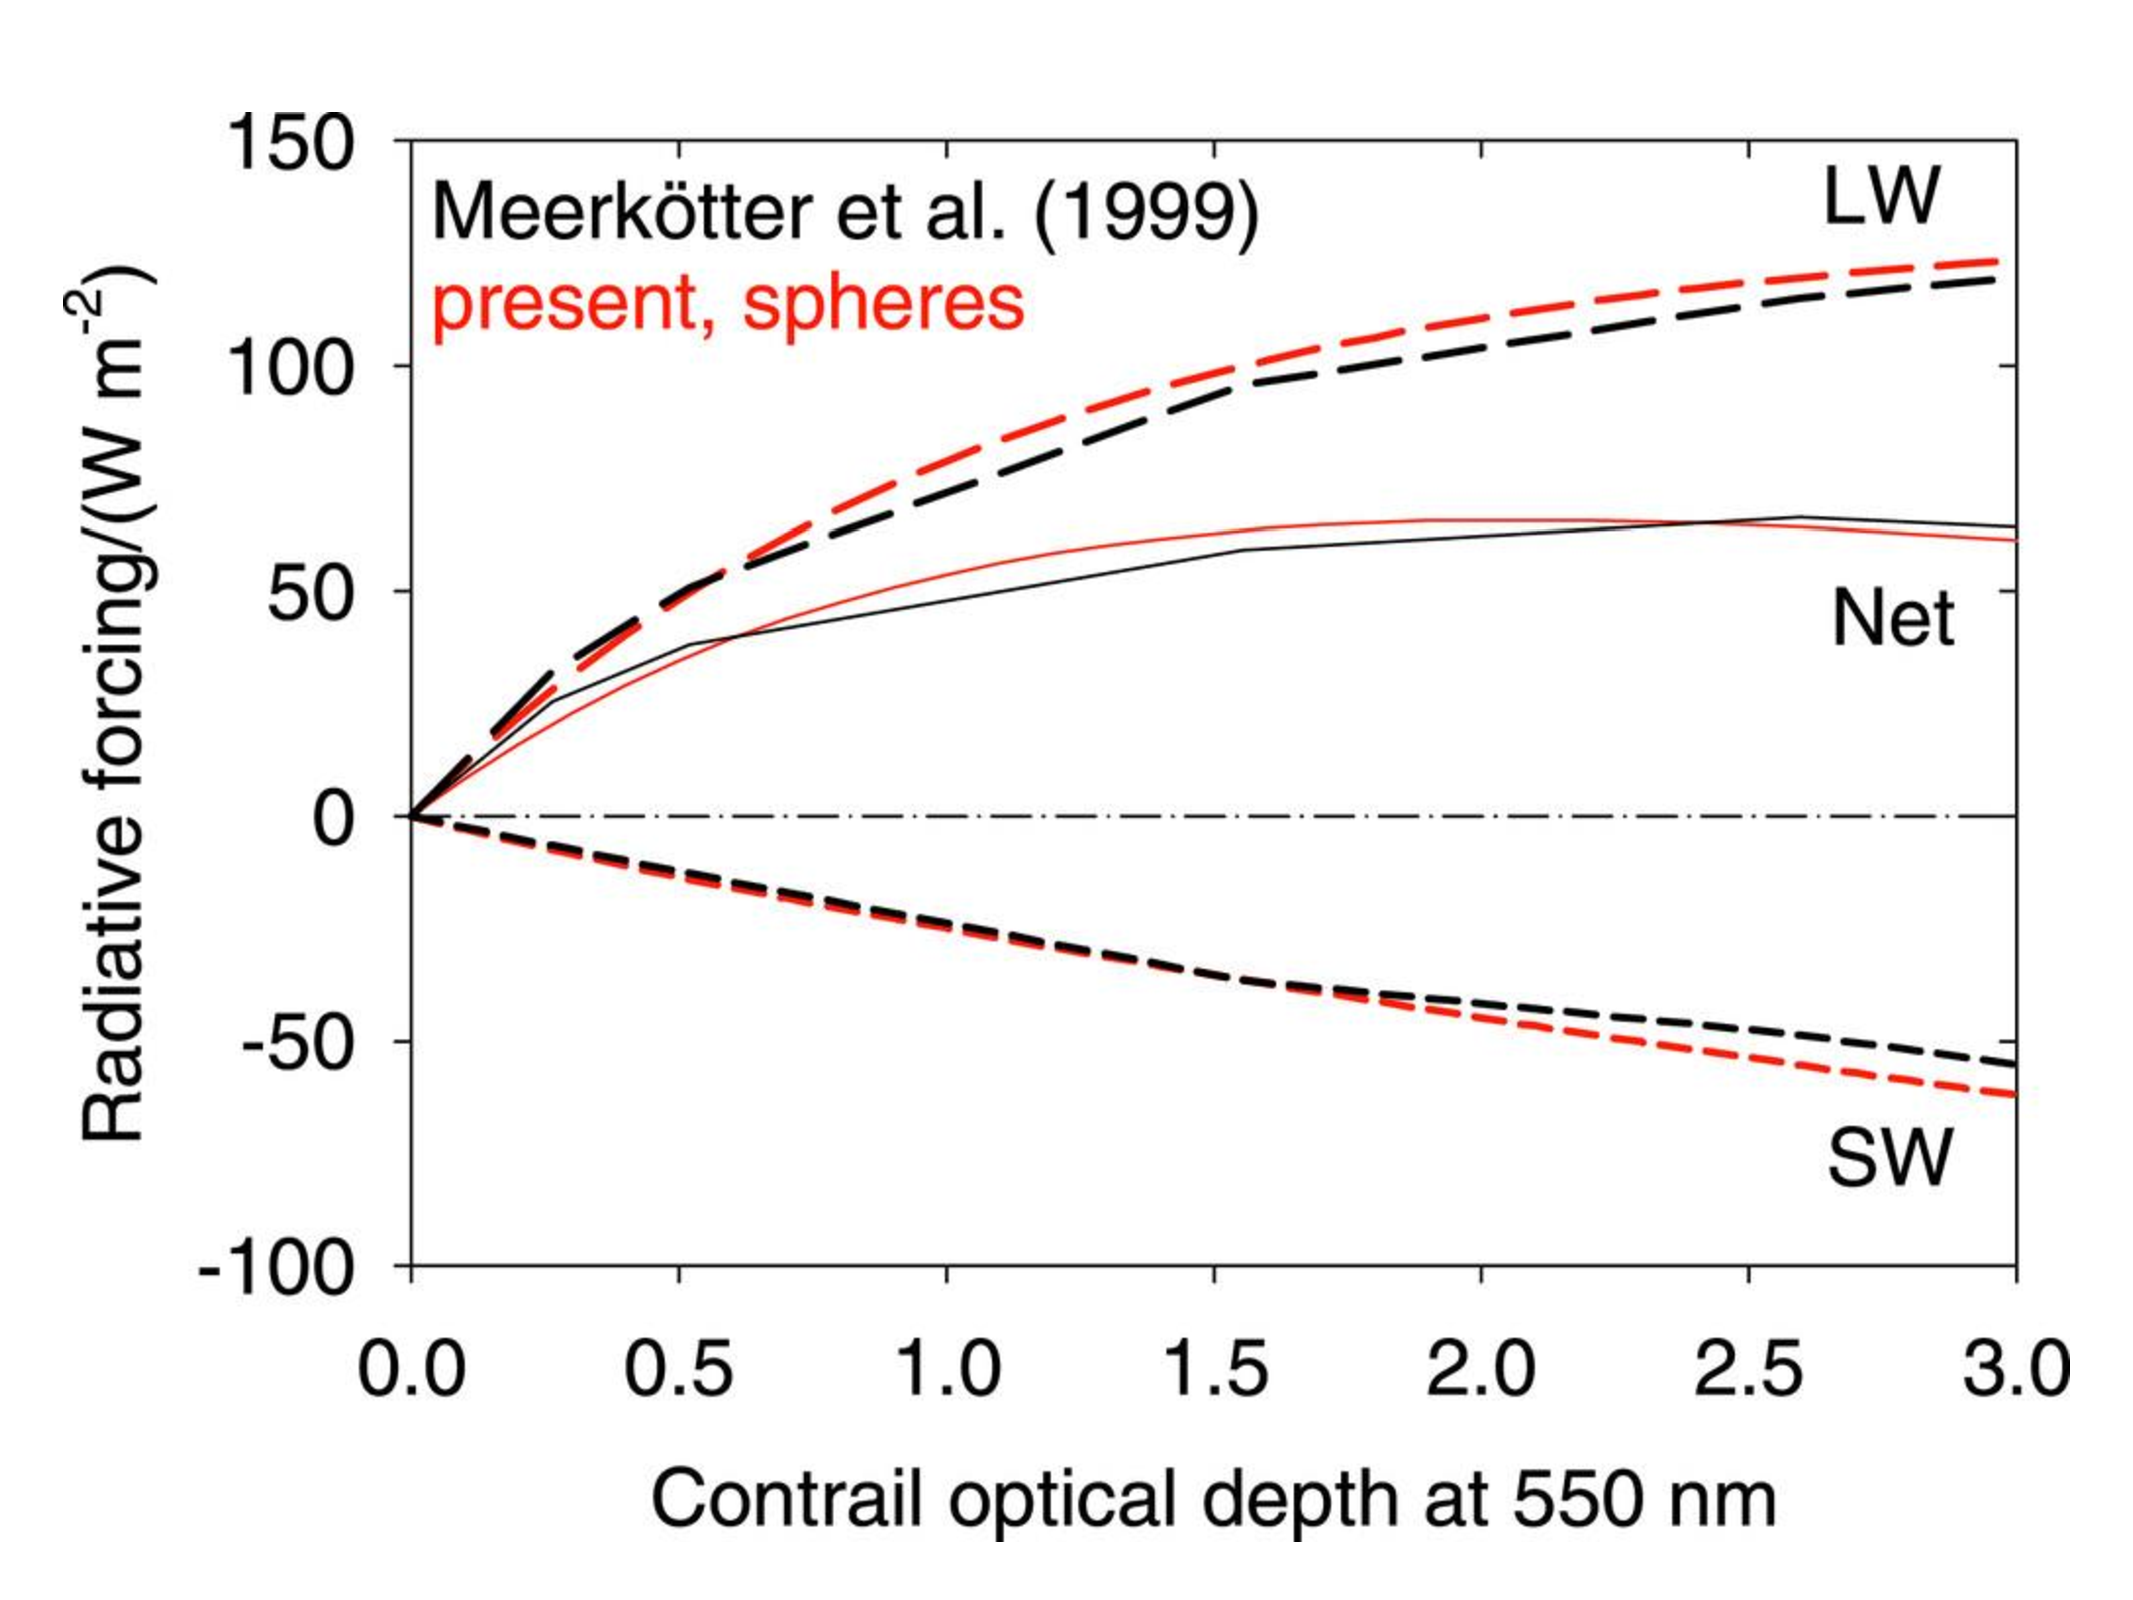
\includegraphics[width=.35\textwidth]{RFvsOD.pdf}
		%\vspace{.2cm}
		\label{RFvsOD}
		}
	\subfloat
		{
		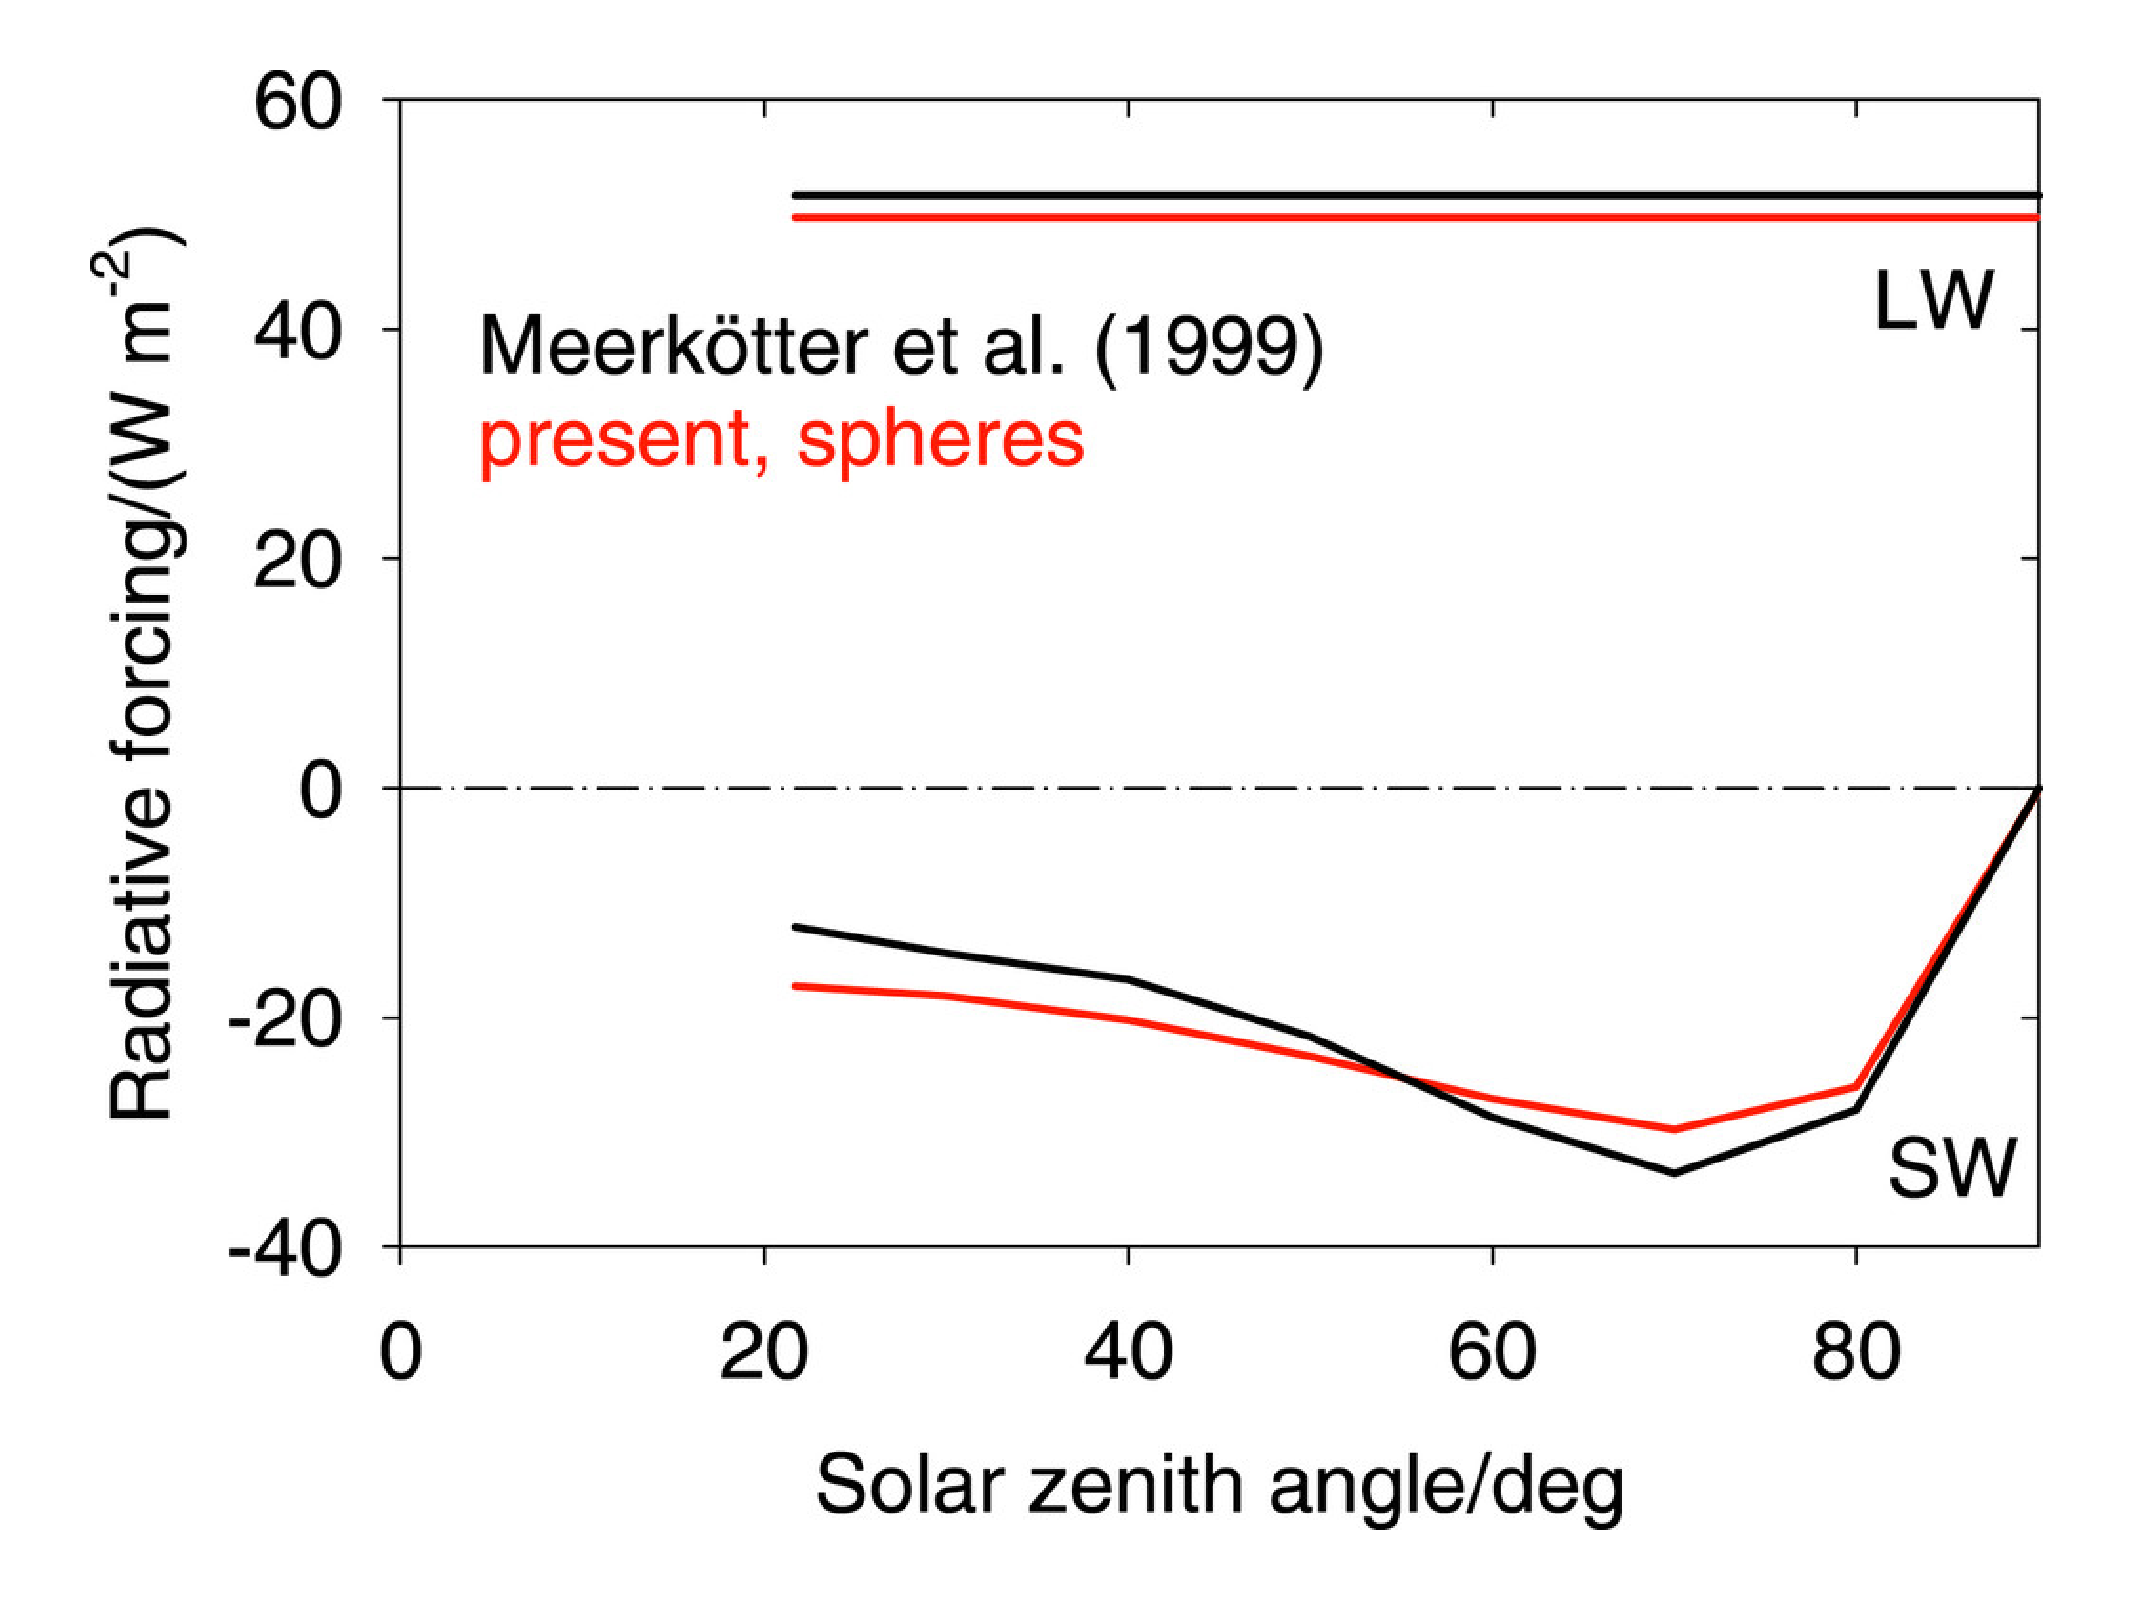
\includegraphics[width=.345\textwidth]{RFvsSZA.pdf}
		\label{RFvsSZA}
		}
	\caption{\textbf{(a)} Daily mean instantaneous SW, LW and net components of RF assuming 100\% contrail cover vs optical depth as calculated using the spherical ice particle model from Schumann et al.\ (2012b) \cite{Schumann2012b}. Results from Meerk{\"o}tter et al.\ (1999) \cite{Meerkotter1999} shown for comparison. \textbf{(b)} RF vs SZA for spherical ice particles, with Meerk{\"o}tter comparison shown. See Schumann et al.\ (2012b) \cite{Schumann2012b} for more detail on assumed atmospheric conditions.}
	\label{}
\end{figure}

Optical depth of contrail cirrus is generally seen to increase radiative forcing, however the relationship is nonlinear and under assumed atmospheric conditions \cite{Meerkotter1999, Schumann2012b}, contrail RF increases with optical depth up to around 2.0, where it peaks, before decreasing at higher optical depths (see figure \ref{RFvsOD}). This is due to the lessening increase of positive LW forcing with increasing optical depth, whilst negative SW forcing continues to drop at a similar rate throughout. In addition to contrail optical properties, the magnitude and direction of contrail forcing is also directly determined by solar position, otherwise known as the solar zenith angle (SZA) (see figure \ref{RFvsSZA}). Throughout the range of SZA values, LW forcing remains constant, because infrared emission from the Earth's surface is unaffected by solar flux. The SW flux on the other hand, goes further negative as SZA increases, up until a maximum at around 70\textdegree. Beyond this, the Sun begins to set and SW forcing returns to zero when the Sun is at 90\textdegree \ to the Earth's surface. This confirms the notion that contrails are solely warming at night, as the positive LW forcing always remains constant, whilst at night there is no chance of negative SW forcing.

\subsection{The saturation of aircraft emissions in high-density airspace regions}
\label{Saturation}
In dense airspace regions, where the frequency of traversing aircraft is high, the resulting exhaust plumes may intersect and overlap, further affecting the nonlinear atmospheric response to chemical and microphysical processing occurring at the plume scale. Two outstanding saturation effects documented in the literature include the surpassing of \ce{NO_x}-saturated conditions and the dehydration of surrounding water vapour due to contrail formation, leading to the mutual inhibition of ice particle growth in the aircraft wake.

\subsubsection{\ce{NO_x}-saturated conditions}
The accumulation of nitrogen oxide emissions in the troposphere due to overlapping aircraft plumes has been observed empirically. For example, Schlager et al.\ (1997) \cite{Schlager1997} witnessed \ce{NO_x} concentrations of up to 30 times the average background concentrations in the North Atlantic Flight Corridor, for an overlap of 2 to 5 aircraft plumes. As discussed in section \ref{Gas_phase_photochem}, the net ozone production rate in the upper troposphere is a nonlinear function of the concentrations of NO and \ce{NO_2}, with increasing \ce{NO_x} leading to increasing \ce{O_3}, up until a maximum, where any additional \ce{NO_x} serves to reduce ozone production efficiency (e.g. figure \ref{NO_x_ozone}). The turnover point, sometimes called the ``compensation point" is determined by competitive reactions involving nitrogen species and \ce{HO_x}. In the \ce{NO_x}-limited regime (left of the minimum ozone production efficiency \ce{P(O_3)_{max}}), NO drives the production of ozone through reaction with the hydroperoxy radical (\ce{HO_2}) \cite{Monks2005}. However, it also drives the removal of \ce{HO_x} through the reaction of OH with \ce{HO_2}, \ce{HNO_4} and \ce{NO_2}, thus limiting \ce{HO_x} available for further \ce{O_3} production \cite{Wennberg1998}. As \ce{NO_x} levels increase up to compensation point, the increasing competition of \ce{HO_x} removal processes begins to level off ozone production efficiency. Beyond this point, further increases in \ce{NO_x} serve to decrease \ce{P(O_3)}, thus signalling the start of the \ce{NO_x}-saturated regime. 

\begin{figure}[H]
  \centering
  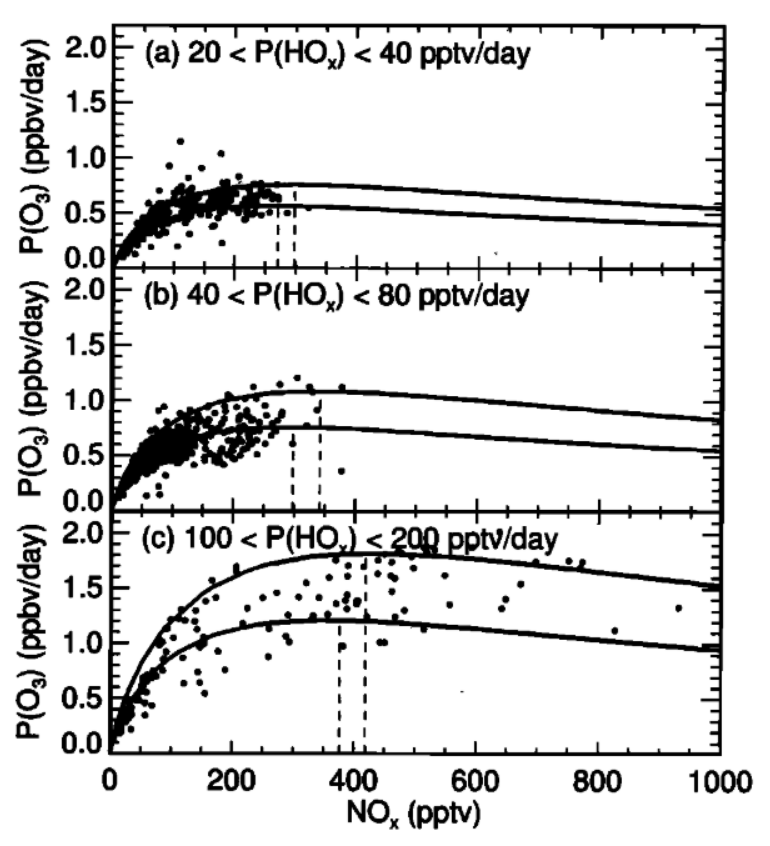
\includegraphics[width=0.5\linewidth]{Jaegle_sat.png}
  \caption{Empirical observations of ozone production rate as a function of \ce{NO_x} concentrations (parts per trillion volume, pptv), for three ranges of primary \ce{HO_x} production: (a) 20--40~pptv/day, (b) 40--80 pptv/day, and (c) 100--200~pptv/day. Solid lines represent the range limits from model calculations. Dashed lines depict the \ce{NO_x} level that induces peak ozone response \cite{Jaegle1999}.}
  \label{Jaegle_sat}
\end{figure}

During the POLINAT/SONEX campaign, Jaegl\'{e} et al.\ (1999) \cite{Jaegle1999} presented the first empirical evidence of \ce{NO_x}-saturated conditions in the NAFC. As seen in figure \ref{Jaegle_sat}, \ce{P(O_3)} levels increased with increasing \ce{NO_x} up until the saturation point, beyond which ozone production begins to drop off. 

As seen in figure \ref{Jaegle_sat} at 100--200~pptv/day of \ce{HO_x} production, \ce{P(O_3)} levels increased with increasing \ce{NO_x} up until around 300~pptv, where it is clear that \ce{NO_x} saturation has been reached. This means that any further emission of \ce{NO_x} under those specific atmospheric conditions will potentially serve to decrease the net ozone production rate. Generally speaking, ozone production efficiency, and hence the threshold for \ce{NO_x}-saturated conditions, is largely dependent on just two variables: the ambient \ce{NO_x} concentration (including the accumulation of \ce{NO_x} from lingering aircraft plumes) and the \ce{HO_x} production rate (which depends on the chemical composition of the atmosphere and the solar intensity \cite{Monks2005}) \cite{Jaegle2001}. 

Furthermore, model results from Kraabol et al. (2000b) \cite{Kraabol2000b} in a study observing interactions between plumes revealed that, for aircraft flying along the same track, plumes of follower aircraft exhibit a considerably smaller ozone response than that of the leader aircraft. This observation on a local scale opens up the discussion for controlled saturation of emissions through formation flight, to take advantage of effects that are beneficial to the climate.

\subsubsection{Dehydration effects due to contrail formation}
Contrails grow and persist in the atmosphere through deposition of water vapour from ice-supersaturated layers of the atmosphere. The conversion of atmospheric water vapour to solid phase ice particles has the potential to deplete local water vapour concentrations in regions conducive to persistent contrail generation \cite{Unterstrasser2010}. It is thought that the depositional growth of contrail cirrus in regions of high airspace density can even lead to the dehydration of \ce{H_2O} at typical flight levels, followed by the redistribution of humidity to lower levels, due to sedimentation and advection processes \cite{Schumann2015}. 

Contrail dehydration effects were first quantified by Burkhardt and K\"{a}rcher (2011) \cite{Burkhardt2011}, in which a global atmospheric model was used to perform long-term integrations of the global impact of contrail cirrus on natural cirrus reduction due to ambient water vapour depletion. The paper found initial RF estimates to be -7~\ce{mWm^{-2}}, lessening the contrail cirrus RF estimate by a factor of approximately one fifth, however the results were not conclusive. Schumann et al.\ (2015) \cite{Schumann2015} furthered this investigation through quantification of the impact of water exchange on contrail properties, large-scale humidity and the background climate. The results suggested that the drying at flight levels caused contrails to become thinner and last longer in the atmosphere, and the net reduction in contrail cirrus RF was deemed to be \textasciitilde15\% (not too dissimilar to the results of the Burkhardt and K{\"a}rcher (2011) \cite{Burkhardt2011}). Furthermore, the results from a second run of the model, with aircraft emissions enhanced by 100 times, showing increasingly significant dehydration effects due to contrail cirrus formation and the redirection of humidity to lower flight levels. This implies that local dehydration effects will be far more significant in dense airspace regions where emissions accumulate and contrails can overlap, such as over mainland areas and in flight corridors. Work by Unterstrasser \cite{Unterstrasser2010, Unterstrasser2020} has elaborated on this concept of local dehydration, through numerical analysis of contrail growth in close proximity flight scenarios. The studies conclude that aircraft contrails compete for available water vapour, mutually inhibiting growth and leading to a saturation effect which diminishes the contrail of subsequent aircraft travelling through that region. Under proposed formation flight scenarios, the total extinction (optical depth) and total ice mass behind a two-aircraft formation are found to be reduced by 20--50\% and 30--60\% respectively.

The presence of plume-scale effects that are amplified in close-proximity flight scenarios begs the question; can climate beneficial saturation effects such as \ce{NO_x}-saturated regimes and contrail-induced dehydration be exploited for mitigation purposes? Section \ref{Mitigation} explores the concept of formation flight and how these additional climate benefits from emissions saturation may provide further impetus for real-world implementation of these concepts.

\subsection{Parametrisation of plume-scale effects into global models}
Plume modelling methods serve as a useful tool for analysing the chemical and physical evolution of aircraft exhaust plumes throughout their lifetime. However, integrating high-resolution plume data into global atmospheric models is simply unfeasible when a large number of flights, on the order of 100,000--200,000 flights per day \cite{Flightradar24}, must be considered. To counteract this, simpler parametrisations of plume models are used, which capture so-called ``effective emissions" that attempt to correct the ID response of the large-scale model, according to the predicted plume-scale effects and their influence on the eventual climate impact. Parametrising plume-scale climate effects into global atmospheric models that assume instantaneous dispersion is a topic covered extensively in the literature, for both ozone-\ce{NO_x} chemistry \cite{Meijer1997, Paoli2020, Paoli2011, Cariolle2009} and contrail and cloud processes \cite{Burkhardt2009}. 

\subsubsection{Parametrisation of gas-phase chemical conversions}
In Paoli et al.\ (2011) \cite{Paoli2011}, three key concepts are reviewed which enable the parametrisation of nonlinear plume chemistry into ID global models; effective emission indices (EEIs), effective conversion factors (ECFs) and effective reaction rates (ERRs). 

The EEI concept was first theorised in Petry et al.\ (1998) \cite{Petry1998}, in an attempt to account for the difference in concentration evolution of key chemical species between large scale models which assume ID and plume models which account for the entrainment of emissions throughout the plume lifetime. EEIs provide a suitable correction to the original EI of an emitted species, so that the concentration is the same in both models at the end of the plume ``dispersion time" ${t_{\mathrm{ref}}}$, when emissions are fully dispersed into the dimensions of the computational grid cell in which they were released.  

Meijer (2001) \cite{Meijer2001} presents the concept of ECFs which are factors applied to the \ce{NO_x} emission index to account for the increased chemical conversion rate of \ce{NO_x} to nitrogen reservoir species in the plume. Since the total emitted reactive nitrogen (\ce{NO_y}) is chemically conserved throughout the plume lifetime, the amount of \ce{NO_y} throughout the plume lifetime is equal to the amount of \ce{NO_x} emitted initially, and hence the sum of ECFs for \ce{NO_x} and all reservoir species is unity \cite{Vohralik2008}. Thus, the faster in-plume conversion rates lead to a decreased \ce{NO_x} ECF, whilst the ECFs of reservoir species such as \ce{HNO_2} and \ce{HNO_3} increase considerably. As a result, the eventual net ozone production is affected as explained in section \ref{Gas-phase_photochem}, however ECFs vary considerably depending on altitude, latitude and seasonal variation meaning the magnitude and direction of the ozone perturbation is also affected.

% EEI and ECF figures

Despite the widespread use of EEIs and ECFs to parametrise plume-scale gas-phase chemical conversions in past literature, there are a number of known issues that affect accuracy such as mass conservation inconsistencies and poor accounting of local and regional variation in dispersion properties and turbulence. Cariolle et al.\ (2009) \cite{Cariolle2009} attempts to overcome such issues with the ERR concept. ERRs reconstruct the concentrations of the emitted species in the plume by diluting the emission to the resolution of the computational grids cell, while modified reaction rates are used to model reactions with ambient chemical species that occur at the plume scale. Modified reaction rates are introduced by the determination of effective reaction rate constants, which are used to compute secondary species produced in the plume. As a result, ERRs build on the EEI and ECF concepts by ensuring full mass conservation by modulating pre-existing background chemical cycles instead of directly estimating mass change, and they account for chemical transport due to diffusion and turbulence processes that are entirely dependent on location. 

% ERR fig

\subsubsection{Parametrisation of heterogeneous chemistry and microphysics}
Despite there being an extensive number of gas-phase chemistry parametrisations, the same cannot be said for parametrisations of heterogeneous chemistry and microphysics, for modelling aircraft plume-scale climate effects at a global scale. K{\"a}rcher et al. (1998) \cite{Karcher1998} was one of the first studies to explicitly attempt to parametrise heterogeneous reactions and aerosol microphysics in global models. The paper attributed the perturbations to the background aerosol layer (due to aerosol emissions from aircraft) to increasing surface areas and number concentrations of aerosol particles, which subsequently increase heterogeneous reaction rates. Findings from Meilinger et al. \cite{Meilinger2002, Meilinger2005} however, reveal that heterogeneous chemistry effects in dispersing aircraft plumes require special consideration of both the chemical and microphysical interactions, and the dynamical response of the plume itself. In Meilinger et al. (2005) \cite{Meilinger2005}, the Mainz Aircraft Plume Model is used to calculate the response of ozone and nitrogen reservoir species in the plume due to heterogeneous chemistry and microphysical effects. It is found from the modelling results that the impact of heterogeneous chemistry and microphysics on the ozone response at global scales is highly sensitive to local meteorology and the instantaneous state of the atmosphere. Therefore, parametrisation of these effects is much more convoluted than first thought, and due to the relatively minute impact on ozone response ($\pm$0.5\%), it is not unreasonable to disregard these effects in global modelling efforts.

Contrarily, the parametrisation of contrail microphysics into global models is of crucial importance, as contrail radiative forcing is determined primarily by the optical properties of its consituent ice particles. Burkhardt and K{\"a}rcher (2009) \cite{Burkhardt2009} summarise the parametrisations necessary to include contrail radiative forcing in global models; this includes parametrising the factors affecting ice supersaturation, contrail formation and persistence, contrail spreading and ice water content. This led to the development of the process-based contrail cirrus module (CCMod), which was later implemented in the global climate model ECHAM4, for global contrail cirrus radiative forcing analysis \cite{Burkhardt2010, Burkhardt2011, Lee2009}. More recently, a microphysical extension to CCMod was applied and implemented in ECHAM5 \cite{Bickel2020, Bock2016}. Model outputs were used to determine the global effective radiative forcing of contrail cirrus in Lee et al.\ (2021) \cite{Lee2021}, finding that the ERF is more than 50\% smaller than the RF equivalent. This is thought to be due to the reduction in natural cloudiness caused by contrail cirrus dehydration of the surrounding atmosphere, and due to the dependence of contrail climate impact on prevailing air traffic distribution patterns. See Lee et al. (2021) \cite{Lee2021} for more info on the parametrisations of contrail and aerosol microphysics implemented to deduce global ERF estimates.


%The \ce{NO_x} emission index is scaled such that the ratio of emission species $i$ to the emission of total reactive nitrogen (\ce{NO_y}) in the aircraft exhaust plume. 

%ECFs depend on assumed lifetime of the plume in the plume model. Difference in net chemical NOx prod and net chemical O3 prod between exhaust and ambient is largest in first few hours after emission. ECFs categorised by month, hourly emission, latitude, altitude. Sensitivity studies show this is a valid assumption.

%The plume model used to compute EEIs in this study is the SP model coupled with a chemistry mechanism known as CHEST (Chemistry Module for the Lower Stratosphere and Troposphere) \cite{}. Such a model requires consideration of atmospheric parameters and demands complex chemical and physical analysis at plume-scale resolution. Analysis of a large number of flights at such high complexity and fidelity is extremely demanding from a computational standpoint, and gives rise to issues surrounding resolving computations between plume models and global models \cite{}. Therefore, it is much more efficient from a large-scale perspective to apply effective emission corrections to aircraft emission inventories, accounting for nonlinear processing in the plume without vastly exceeding computational limitations.


%\subsection{Limitations to the plume modelling approach}
%Plume scale modelling of aircraft emissions is typically simulated using Eulerian 3-D atmospheric chemistry transport models to investigate its chemical impacts on the environment. However, this approach has also been recognised as a major uncertainty because emissions generally occur in plumes with scales much smaller than the grid resolution. Thus, this approach cannot explicitly capture the high initial concentrations of the chemicals within the plume. To overcome this, the Lagrangian models can be used in a domain-filling mode where the air parcels are distributed in the model domain proportionally to air density and each air parcel carries roughly the same mass of air. Interactions between neighbouring air parcels can be specified to represent mixing. In the grid cells with air flowing into the model domain, mass fluxes are accumulated with time and when the accumulated mass exceeds the mass of the air parcel, a new air parcel is released at a randomly chosen position at the boundary of the box. 

%The plumes in sub-grid scale arises an uncertainty due to the coarse grid resolutions of CTM model.  Such uncertainty can be improved by using grids with very fine resolution emissions and mixing. However, this can increase computational burden due to the large number of grid cells in the model domain as well as smaller time steps. Alternatively, a nested grid approach can be used with employing one or few fine grids over regions of special interest within larger domain. The multiple grid simulations can be performed simultaneously with two-way flow of information between the coarse and fine grids.


% Nested grid modelling

